\documentclass[conference, brazil]{IEEEtran}
\usepackage{graphicx}
\usepackage[pdftex]{hyperref}
\usepackage{caption}
\usepackage{subcaption}
\usepackage{multirow}
\usepackage[portuguese]{babel}

%TODO
%terceiro algoritmo
%OK Explicar bibliotecas
%OK prints e tabelas
%OK hardware e tempo
%OK conclusao
%mais referencias


% correct bad hyphenation here
\hyphenation{op-tical net-works semi-conduc-tor}

\begin{document}

\title{Detecção do Vírus da COVID-19 por Microscopia Eletrônica}    

\author{
\IEEEauthorblockN{Laura N. de Andrade, Lucca A. M. Santos, Richard V. R. Mariano}
%\IEEEauthorblockA{\IEEEauthorrefmark{1}Departamento de Ciência da Computação, Pontifícia Universidade Católica de Minas Gerais (PUC Minas), Belo Horizonte, Brasil}
landrade@sga.pucminas.br, lucca.santos@sga.pucminas.br, richard.mariano@sga.pucminas.br}


% The paper headers
\markboth{Journal of \LaTeX\ Class Files,~Vol.~14, No.~8, August~2015}%
{Shell \MakeLowercase{\textit{et al.}}: Bare Demo of IEEEtran.cls for IEEE Journals}

% make the title area
\maketitle
\begin{abstract}
COVID-19 é uma doença infeciosa causada pelo coronavírus da síndrome respiratória aguda grave 2 (SARS-CoV-2). Este artigo é a documentação do programa desenvolvido para detectar o vírus. Explicamos as técnicas implementadas e as bibliotecas utilizadas. Ao final discutimos os resultados obtidos e os experimentos feitos.

\end{abstract}

\begin{IEEEkeywords}
Vírus, imagem, Transformada de Hough, Correlação Cruzada, Limiarização, COVID-19
\end{IEEEkeywords}


\IEEEpeerreviewmaketitle

\section{Introdução} %descrição do problema
\label{sec:introduction}
\IEEEPARstart{A}{ COVID-19} é uma doença infeciosa causada pelo coronavírus da síndrome respiratória aguda grave 2 (SARS-CoV-2). A doença surgiu no final de 2019 e já atingiu mais de 180 países, com mais de 6 milhões de pessoas infectadas no mundo todo. Este trabalho foi desenvolvido como parte da disciplina de Processamento de Imagens. Desenvolvemos um aplicativo para realizar a detecção do vírus em imagens, utilizando técnicas diversas, além de realizar a contagem de vírus contidos naquela imagem. 

\section{Motivação}
\label{sec:relatedwork}
A motivação deste trabalho foi colocar em prática o conhecimento adquirido durante o semestre, além de trabalhar um assunto de importância mundial.

\section{Objetivos}
\label{sec:design}
Este trabalho tem como objetivo identificar o coronavírus em meio a várias células a partir da análise de uma imagem aplicando métodos de reconhecimento de padrões e aprendizado de máquina.

\section{Técnicas implementadas}
\label{sec:design}

Para o desenvolvimento desta aplicação foi implementada uma interface gráfica de fácil utilização e manutenção. Dentre as linguagens propostas (C, C++ ou Java), foi escolhida para desenvolver a aplicação a linguagem Java devido a familiaridade e a facilidade de encontrar materiais, como bibliotecas e fóruns, para auxiliar na criação do projeto. Utilizamos diversas bibliotecas da linguagem na implementação, como por exemplo \textit{OpenCV}. %Buscas artigo 

A janela inicial do sistema possui 8 funcionalidades. São elas: Carregamento de imagem, Seleção, \textit{Zoom In}, \textit{Zoom Out}, Restauração de imagem, Limiarização, Rotulação e Detecção, cada uma representada por um botão.

\begin{enumerate}
\item\textbf{Carregamento de imagem} - Ao selecionar essa opção, uma janela se abrirá para que você escolha a imagem a ser carregada, em um dos seguintes formatos: PNG, TIFF ou JPG. Após escolher, a imagem é carregada e exibida na tela, e automaticamente um histograma de tons de cinza é calculado. Um histograma mostra a frequência com que um certo valor aparece na amostra. Neste caso, quantas vezes um tom de cinza aparece na imagem escolhida.
\item\textbf{Seleção} - Com esta ferramenta o usuário pode selecionar uma área da imagem. Deve-se clicar em dois pontos, que formaram um retângulo que indica a seleção. A seleção deve ser um exemplo do coronavírus para que a partir dele se possa identificar os outros vírus.
\item\textbf{Zoom In} - Esta aplicação permite que você escolha, através de uma caixa de diálogo, o percentual de zoom que deseja aplicar na imagem.
\item\textbf{Zoom Out} - Análogo ao "Zoom In", porém distancia a imagem.
\item\textbf{Restauração de imagem} - Esta funcionalidade tem como único objetivo restaurar a imagem original caso tenha sido anteriormente limiarizada ou rotulada.
\item\textbf{Limiarização} - A limiarização só pode ser usada quando alguma imagem foi carregada anteriormente. Um algoritmo binário é aplicado, dividindo toda a cor da imagem em apenas dois tons, preto e branco. A partir de uma barra de \textit{slider}, o usuário pode alterar o ponto desta divisão.
\item\textbf{Rotulação} - Uma rotulação só é possível quando a imagem já foi limiarizada previamente, dessa forma, caso a imagem não esteja limiarizada, a rotulação aciona a função de limiarização e depois rotula. Ela colore cada objeto de uma cor, e o fundo de outra, permitindo assim, a identificação mais precisa de cada objeto.
\item\textbf{Detecção} - Essa função só é liberada após o usuário selecionar na imagem o exemplo de um vírus. Sua única ação é iniciar uma nova janela onde os algoritmos de detecção serão utilizados.

\end{enumerate}

% não necessariamente precisa ser esses algoritmos, podemos trocar depois
A segunda janela, que é chamada pelo botão de detecção, possui 2 funcionalidades. Algoritmos de Transformada de Hough Elíptica e Correlação Cruzada, cada uma representada por um botão que ao clicado executa o algoritmo e exibe o resultado na tela.

\begin{enumerate}
    \item\textbf{Transformada de Hough Elíptica}: A transformada de Hough é uma técnica usada para extração de características, usada na análise de imagens, visão computacional e processamento de imagem digital. O objetivo do algoritmo é encontrar formas geométricas em imagens, como retas, círculos e elipses.
    
    \item\textbf{Correlação Cruzada}: A correlação cruzada é um artifício usado em processamento de imagens digitais para encontrar, na imagem sendo processada, pedaço(s) que equivalem a uma imagem usada como \textit{template}.
    

\end{enumerate}


\section{Bibliotecas}
\label{sec:design}
As bibliotecas utilizadas para o desenvolvimento da aplicação foram:
\begin{itemize}
\item \textit{Java Swing}: Interface (\textit{frames}, painéis, botões, \textit{label}).

\item \textit{Java AWT}: Captura de eventos.

\item \textit{OpenCV~\cite{opencv}}: Uma biblioteca desenvolvida em C++, mas está disponível para diversas linguagens de programação, como C, Python, GO e Java. Ela possui as funções de processamento de imagens que utilizamos nos algoritmos de detecção do coronavírus.

\item \textit{Luminance~\cite{Luminance}}: Biblioteca utilizada na limiarização. Calcula a luminância de cada pixel para garantir uma limiarização mais eficiente.
\end{itemize}



\section{Algoritmos}
\label{sec:Algoritmos}
Ao carregar a imagem, um histograma com os tons de cinza é calculado e exibido na tela. Algumas funcionalidades estão disponíveis para uma melhor análise. Temos o \textit{Zoom}, que é uma funcionalidade mais simples, mas que permite um aumento, ou redução da imagem. A limiarização traz novas possibilidades ao dividir a imagem em dois tons, permitindo uma melhor identificação do que é fundo e do que é objeto. Na Limiarização um slide bar está disponível para definir o limite do tom para separação binária, assim, tudo que fica a baixo desse valor fica preto, e tudo acima fica branco. A partir disso, temos a rotulação que em uma imagem limiarizada, é capaz de separar através de cores, os objetos identificados na imagem.

Ao selecionar a parte da imagem que contém o vírus, o próximo passo é clicar no botão detectar para abrir a janela de detecção. Nessa janela existe um botão para cada algoritmo implementado e 2 \textit{sliders} para variar parâmetros nas funções. A área selecionada e a limiarização aplicada influenciam diretamente na eficiência dos algoritmos.

Na Transformada de Hough~\cite{HoughCircle}, utilizando a biblioteca OpenCV, primeiro encontramos todas as circunferências. É aplicado um filtro de suavização na imagem para também encontrar outras formas, como elipses. Com todas as formas armazenadas, comparamos os tons de cinza de cada elipse com a área selecionada previamente. A porcentagem de aceitação (vírus/não vírus) para essa comparação é definida pelo usuário diretamente através da barra de slide "Máxima diferença" que varia de 0 a 50\%. Se a diferença de tons de cinza entre a área selecionada e a elipse em questão for menor que a máxima diferença, então o objeto é um vírus.

A Correlação Cruzada~\cite{TemplateMatching} também utiliza a biblioteca OpenCV para buscar áreas de possíveis vírus. Nesse caso, o algoritmo busca pela área mais semelhante a selecionada. Para melhorar a eficiência do algoritmo foi implementado um sistema de iterações. A cada iteração é removido da imagem o recorte que tenha maior similaridade à área selecionada, dessa forma encontra-se vários vírus distintos. Para definir o número de iterações, e consequentemente a quantidade de possíveis vírus a serem encontrados, se utiliza uma barra de \textit{slider} chamada "Número máximo de vírus" que varia de 0 ao tamanho da imagem divida pelo tamanho do \textit{template} (área selecionada). Após isso, comparamos os tons de cinza de cada potencial área com o \textit{template}. Assim como a transformada de Hough, a porcentagem de aceitação para essa comparação também é definida pelo usuário através da barra de slide "Máxima diferença" que varia de 0 a 50\%.


\section{Experimentos e Resultados}
\label{sec:Experimentos e Resultos}
Os algoritmos desenvolvidos mostraram um ótimo desempenho na solução do problema, como podemos ver nas figuras \ref{fig1} e \ref{fig2}. Estes resultados dependem da melhor escolha de parâmetros e área de seleção.

%adicinar os boxplot
\begin{figure}[htpb]
\centering
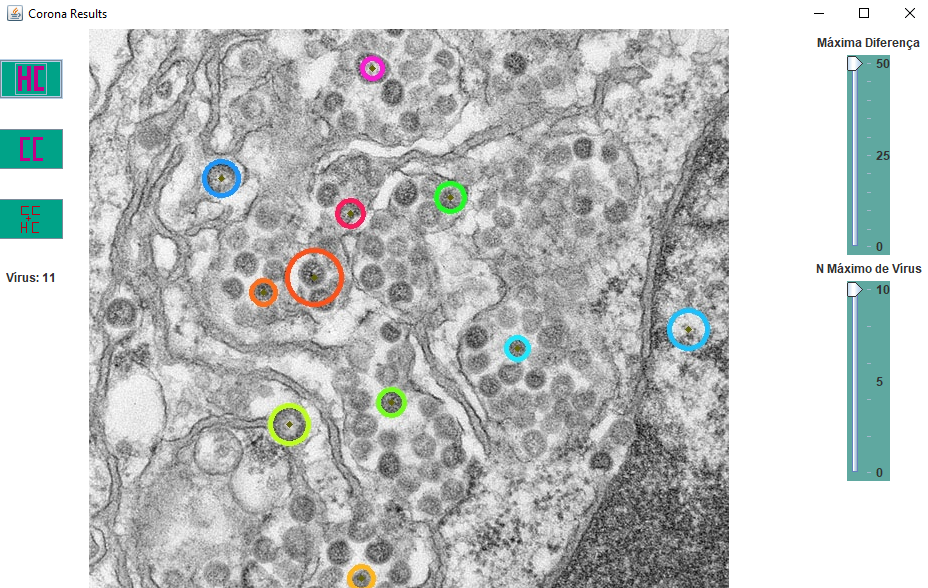
\includegraphics[scale=0.4]{THE.png}
\caption{Demonstração do funcionamento do algoritmo Transformada de Hough Elíptica}
\label{fig1}
\end{figure}

\begin{figure}[htpb]
\centering
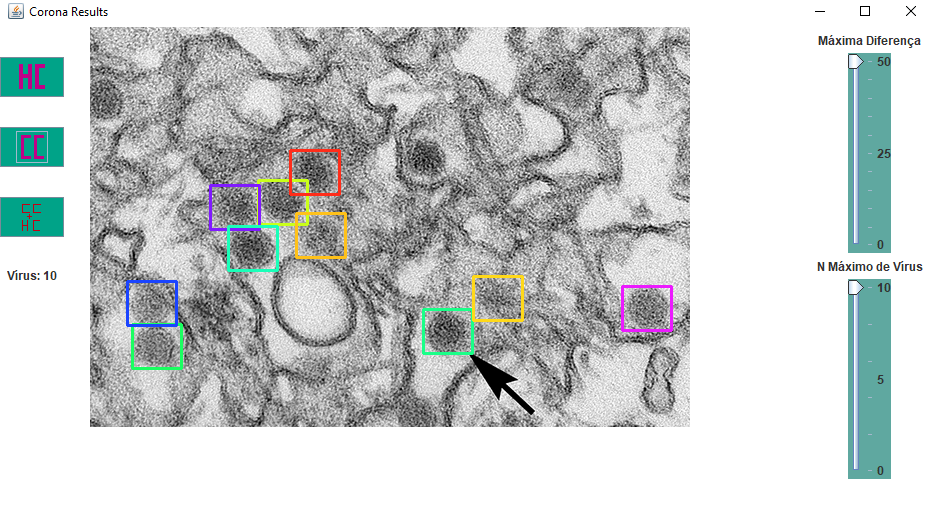
\includegraphics[scale=0.4]{CC.png}
\caption{Demonstração do funcionamento do algoritmo Correlação Cruzada}
\label{fig2}
\end{figure}

Para evitar \textit{overfitting} executamos uma série de testes com várias possibilidades e comparamos os resultados. As tabelas \ref{table1} e \ref{table2} mostram o resultado obtido. 

Na montagem da tabela, fizemos uma análise através da nossa observação do que se encaixaria como vírus.

\begin{table}[htpb]
\centering
\caption{Transformada de Hough Elíptica}
\begin{tabular}
{|c|c|c|c|c|}
\hline
Máx. diferença & Img & Nº de vírus & Corretos & Falso positivo\\
\hline
50 & 1 & 11 & 10 & 1\\
\hline
40 & 1 & 8 & 7 & 1\\
\hline
30 & 1 & 2 & 2 & 0\\
\hline
50 & 2 & 6 & 6 & 0\\
\hline
40 & 2 & 2 & 2 & 0\\
\hline
30 & 2 & 0 & 0 & 0\\
\hline
\end{tabular}
\label{table1}
\end{table}

\begin{table}[htpb]
\centering
\caption{Correlação Cruzada}
\begin{tabular}
{|c|c|c|c|c|c|}
\hline
Máx. dif. & Máx. vírus & Img & Nº de vírus & Corretos & F. positivo\\
\hline
50 & 10 & 1 & 9 & 5 & 4\\
\hline
50 & 5 & 1 & 5 & 3 & 2\\
\hline
25 & 10& 1 & 4 & 4 & 0\\
\hline
25 & 5 & 1 & 2 & 2 & 0\\
\hline
50  & 10 & 2 & 10 & 8 & 2\\
\hline
50  & 5 & 2 & 5 & 5 & 0\\
\hline
25 & 10 & 2 & 8 & 6 & 2\\
\hline
25 & 5 & 2 & 3 & 3 & 0\\
\hline
\end{tabular}
\label{table2}
\end{table}

Durante o desenvolvimento deste trabalho, foi possível perceber que cada algoritmo funciona melhor para um determinado tipo de imagem. No caso da Transformada de Hough Elíptica, descobrimos que seu desempenho é melhor quando as formas a serem detectadas possuem uma borda mais definida.

Já a Correlação Cruzada, detecta formas com uma forma mais próxima da forma do pedaço da imagem usado como \textit{template}. O principal problema deste algoritmo é que ele identifica somente formas de mesmo tamanho, logo, se tivermos um objeto extremamente parecido com a área selecionada, mas de dimensão diferente, o algoritmo não é capaz de encontrar.

\section{Hardware}
\label{sec:applications}
O computador utilizado para os testes e a execução do programa foi um Thinkpad t440s, com um processador Intel Core i7-4600 (quarta geração), memória RAM de 8,00GB (7,88 utilizáveis). O sistema operacional da máquina é um Windows 10 Home edition.

%CPU 2.10GHz 2.69 GHz.

Neste \textit{hardware} nenhuma das funcionalidades da aplicação atingiram um tempo superior a 1 segundo de execução.

\section{Conclusão e Trabalhos Futuros}
\label{sec:conclusion}
Os algoritmos de detecção se mostraram promissores na resolução do problema proposto de identificação do coronavírus. O objetivo inicial de colocar em uso o conhecimento adquirido durante o semestre foi atingido e aperfeiçoado, uma vez que foi possível visualizar através de experimentos práticos o que antes era somente teórico.

Posteriormente, existem melhoras que podem ser feitas a ambos algoritmos, para que o resultado obtido seja o mais próximo possível do esperado, novos algoritmos podem ser propostos como LBPH e Descritores de Haralick, além da união de métodos de cada algoritmo para buscar uma melhor performance.
  
A resolução encontrada para o algoritmo de Rotulação também pode ser melhorada no futuro, limpando as bordas dos objetos e consequentemente obtendo um esqueleto mais definido, levando a uma melhor rotulação da imagem.

Por fim, o algoritmo de Limiarização, apresentou um desempenho excelente em todas as imagens utilizadas para os testes.


%\begin{thebibliography}{7}
%\end{thebibliography}

\bibliographystyle{ieeetr}
\bibliography{refs}
\end{document}